% ------------------------------------------------------------------------
% ------------------------------------------------------------------------
% abnTeX2: Modelo de Projeto de pesquisa em conformidade com 
% ABNT NBR 15287:2011 Informação e documentação - Projeto de pesquisa -
% Apresentação 
% ------------------------------------------------------------------------ 
% ------------------------------------------------------------------------

\documentclass[
	% -- opções da classe memoir --
	12pt,				% tamanho da fonte
	%openright,			% capítulos começam em pág ímpar (insere página vazia caso preciso)
	oneside,			% para impressão em verso e anverso. Oposto a oneside
	a4paper,			% tamanho do papel. 
	% -- opções da classe abntex2 --
	%chapter=TITLE,		% títulos de capítulos convertidos em letras maiúsculas
	%section=TITLE,		% títulos de seções convertidos em letras maiúsculas
	%subsection=TITLE,	% títulos de subseções convertidos em letras maiúsculas
	%subsubsection=TITLE,% títulos de subsubseções convertidos em letras maiúsculas
	% -- opções do pacote babel --
	english,			% idioma adicional para hifenização
	french,				% idioma adicional para hifenização
	spanish,			% idioma adicional para hifenização
	brazil,				% o último idioma é o principal do documento
	]{abntex2}

% ---
% PACOTES
% ---

% ---
% Pacotes fundamentais 
% ---
\usepackage{lmodern}			% Usa a fonte Latim Moderno
\usepackage[T1]{fontenc}		% Selecao de codigos de fonte.
\usepackage[utf8]{inputenc}		% Codificação do documento (conversão automática dos acentos)
%\usepackage{indentfirst}		% Indenta o primeiro parágrafo de cada seção.
\usepackage{color}				% Controle das cores
\usepackage{graphicx}			% Inclusão de gráficos
\usepackage{microtype} 			% para melhorias de justificação
\usepackage[T1]{fontenc}
% ---
%\usepackage{subcaption} 

% ---
% Pacotes adicionais, usados apenas no âmbito do Modelo Canônico do abnteX2
% ---
%\usepackage{lipsum}				% para geração de dummy text
% ---

% ---
% Pacotes de citações
% ---
\usepackage[brazilian,hyperpageref]{backref}	 % Paginas com as citações na bibl
\usepackage[alf]{abntex2cite}	% Citações padrão ABNT

% --- 
% CONFIGURAÇÕES DE PACOTES
% --- 

% ---
% Configurações do pacote backref
% Usado sem a opção hyperpageref de backref
\renewcommand{\backrefpagesname}{Citado na(s) página(s):~}
% Texto padrão antes do número das páginas
\renewcommand{\backref}{}
% Define os textos da citação
\renewcommand*{\backrefalt}[4]{
	\ifcase #1 %
		Nenhuma citação no texto.%
	\or
		Citado na página #2.%
	\else
		Citado #1 vezes nas páginas #2.%
	\fi}%
% ---

% ---
% Informações de dados para CAPA e FOLHA DE ROSTO
% ---
\titulo{Análise de Dados da Covid-19 na cidade de Dourado, MS:\\ um estudo descritivo e comparativo  da situação do município}

\autor{Fernando Ferraz Ribeiro}
\local{Salvador, Bahia, Brasil}
\data{Junho, 2020}
\instituicao{%
  Universidade Federal da Bahia - UFBA
  \par
  Faculdade de Arquitetura
  \par
  PPG-AU}
\tipotrabalho{Relatório Técnico}
% O preambulo deve conter o tipo do trabalho, o objetivo, 
% o nome da instituição e a área de concentração 
\preambulo{}
% ---

% ---
% Configurações de aparência do PDF final

% alterando o aspecto da cor azul
\definecolor{blue}{RGB}{41,5,195}

% informações do PDF
\makeatletter
\hypersetup{
     	%pagebackref=true,
		pdftitle={\@title}, 
		pdfauthor={\@author},
    	pdfsubject={\imprimirpreambulo},
	    pdfcreator={LaTeX with abnTeX2},
		pdfkeywords={Análise de dados}{Covid-19}{Dourados-MS}, 
		colorlinks=true,       		% false: boxed links; true: colored links
    	linkcolor=blue,          	% color of internal links
    	citecolor=blue,        		% color of links to bibliography
    	filecolor=magenta,      		% color of file links
		urlcolor=blue,
		bookmarksdepth=4
}
\makeatother
% --- 

% --- 
% Espaçamentos entre linhas e parágrafos 
% --- 

% O tamanho do parágrafo é dado por:
\setlength{\parindent}{0cm}

% Controle do espaçamento entre um parágrafo e outro:
\setlength{\parskip}{0.2cm}  % tente também \onelineskip

% ---
% compila o indice
% ---
\makeindex
% ---

% ----
% Início do documento
% ----
\begin{document}

% Retira espaço extra obsoleto entre as frases.
\frenchspacing 

% ----------------------------------------------------------
% ELEMENTOS PRÉ-TEXTUAIS
% ----------------------------------------------------------
\pretextual

% ---
% Capa
% ---
\imprimircapa
% ---

% ---
% Folha de rosto
% ---
\imprimirfolhaderosto
% ---
 

% ---
% NOTA DA ABNT NBR 15287:2011, p. 4:
%  ``Se exigido pela entidade, apresentar os dados curriculares do autor em
%     folha ou página distinta após a folha de rosto.''
% ---

% ---
% inserir lista de ilustrações
% ---
%\pdfbookmark[0]{\listfigurename}{lof}
%\listoffigures*
%\cleardoublepage
% ---

% ---
% inserir lista de tabelas
% ---
%\pdfbookmark[0]{\listtablename}{lot}
%\listoftables*
%\cleardoublepage
% ---

% ---
% inserir lista de abreviaturas e siglas
% ---
% \begin{siglas}
%   \item[Fig.] Area of the $i^{th}$ component
%   \item[456] Isto é um número
%   \item[123] Isto é outro número
%   \item[lauro cesar] este é o meu nome
% \end{siglas}
% ---

% ---
% inserir lista de símbolos
% ---
% \begin{simbolos}
%   \item[$ \Gamma $] Letra grega Gama
%   \item[$ \Lambda $] Lambda
%   \item[$ \zeta $] Letra grega minúscula zeta
%   \item[$ \in $] Pertence
% \end{simbolos}
% ---

% ---
% inserir o sumario
% ---
\pdfbookmark[0]{\contentsname}{toc}
\tableofcontents*
\cleardoublepage
% ---


% ----------------------------------------------------------
% ELEMENTOS TEXTUAIS
% ----------------------------------------------------------
\textual

% ----------------------------------------------------------
% Introdução
% ----------------------------------------------------------
\chapter{Introdução}

Nas últimas décadas, a quantidade de dados produzidos pela humanidade cresceu de forma exponencial. A aquisição, manipulação, gestão, armazenamento e criação de valor a partir destes dados, através de ambientes computacionais, tem-se apresentado como um novo paradigma tecnológico da humanidade. Este campo disrruptivo do conhecimento recebeu a denominação de Ciência de Dados, conceito que envelopa alguns termos frequentemente associados à inovação científica, técnica e social como \emph{Big Data}, mineração de dados, \emph{Business Intelligence} internet das coisas, inteligência artificial e aprendizado de máquina, dentre outros \cite[p. 12-13]{EMCdata2015}. Na subárea dos dados geoespaciais, embora carregue características específicas importantes, a mudança tem apresentado escala semelhante. Áreas como o planejamento urbano, \cite{OSMAN2019620, Zhou2016}, o monitoramento e gestão do trânsito de veículos \cite{Bermudez-Edo2018}, políticas públicas e serviços para a cidade, seus habitantes e visitantes \cite{Lim2018}, tem sofrido grande influência da Ciência de Dados, promovida por universidades, centros de pesquisa, empresas e poder público.

O que se propõe neste projeto de pesquisa é a condução de uma análise da mobilidade na Cidade de Salvador a partir da manipulação, estudo, análise e combinação de dados e informações de três bancos de dados distintos. 


\begin{figure}[!htb]
	\centering
	\caption{legenda}
	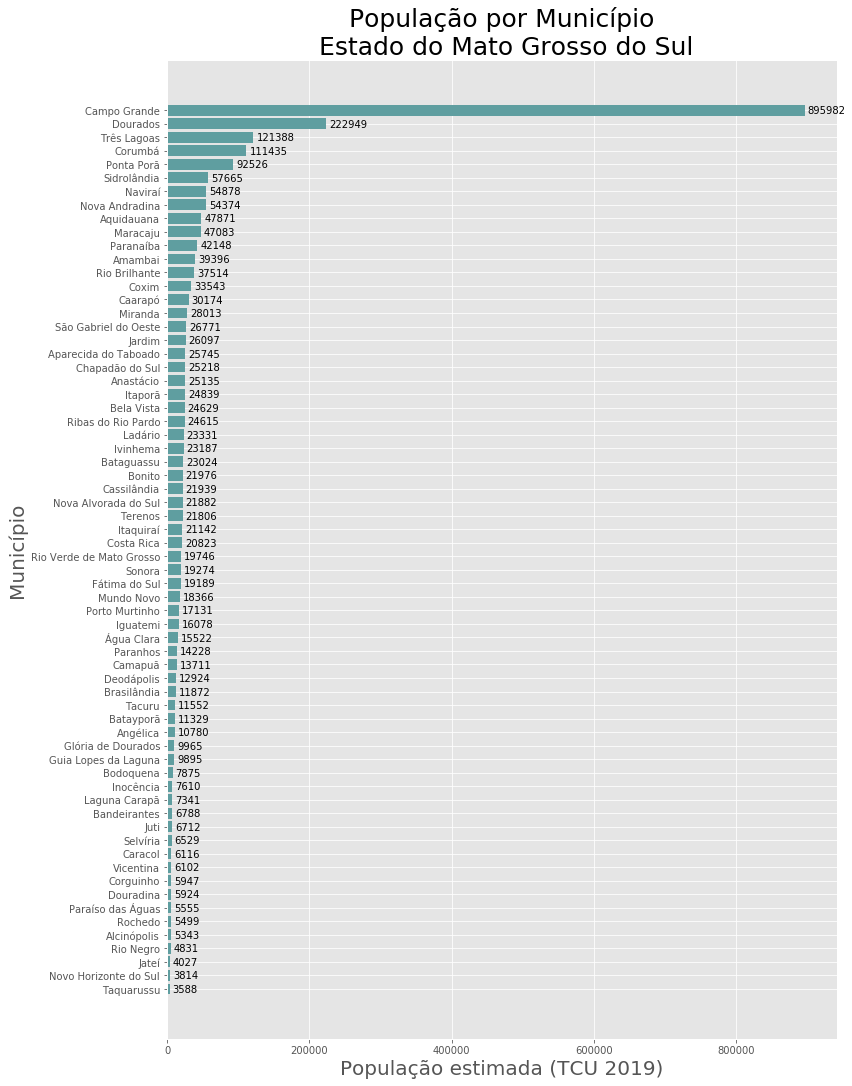
\includegraphics[width=1
	\textwidth]{./figs/pop_por_municipio.png}
	\\{\footnotesize Fonte: Elaborada Pelos Autores}
	\label{fig:teste}
\end{figure}

% ----------------------------------------------------------
% Desenvolvimento
% ----------------------------------------------------------
\chapter{Ciência de Dados e Planejamento Urbano}
\section{Objeto de Estudo e Abordagem Teórica}
\section{Justificativa}
\section{Objetivos}
\section{Metodologia}
\chapter{Cronograma}

% ----------------------------------------------------------
% Conclusão
% ----------------------------------------------------------
\chapter{Considerações finais}

% ----------------------------------------------------------
% ELEMENTOS PÓS-TEXTUAIS
% ----------------------------------------------------------
\postextual
% ----------------------------------------------------------
% Referências bibliográficas
% ----------------------------------------------------------
\bibliography{abntex2-modelo-references}
% ----------------------------------------------------------
% Fim do documento
% ----------------------------------------------------------
\end{document}
